\documentclass[10pt]{article}\usepackage[]{graphicx}\usepackage[]{color}
%% maxwidth is the original width if it is less than linewidth
%% otherwise use linewidth (to make sure the graphics do not exceed the margin)
\makeatletter
\def\maxwidth{ %
  \ifdim\Gin@nat@width>\linewidth
    \linewidth
  \else
    \Gin@nat@width
  \fi
}
\makeatother

\usepackage{Sweavel}


\usepackage{hyperref,url}
\usepackage[a4paper]{geometry}
\usepackage{a4wide}
\usepackage{float}
\usepackage[english]{babel}
\usepackage[utf8]{inputenc}
\usepackage{csquotes}
\usepackage{amsmath}
\usepackage{amssymb}
\usepackage{xspace}
\usepackage[numbers]{natbib}
\bibliographystyle{unsrtnat}
\usepackage{subcaption}
\usepackage[font={small}]{caption}
\usepackage{booktabs}
\usepackage{listings}
\usepackage{cleveref}
\usepackage{lipsum}
\usepackage{graphicx}
\usepackage{epstopdf}
\graphicspath{{../figures/}}
\epstopdfsetup{outdir=./}
\newcommand{\approxtext}[1]{\ensuremath{\stackrel{\text{#1}}{=}}}
\newcommand{\matr}[1]{\mathbf{#1}}
\newcommand{\partt}[2]{\ensuremath{\dfrac{\partial {#1}}{\partial {#2}}}}
\renewcommand{\d}[1]{\ensuremath{\operatorname{d}\!{#1}}} % non-italized differentials
\newcommand{\h}[0]{\ensuremath{\hbar}} % hbar
\newcommand{\avg}[1]{\ensuremath{\langle {#1} \rangle}} % hbar

\def\changemargin#1#2{\list{}{\rightmargin#2\leftmargin#1}\item[]}
\let\endchangemargin=\endlist 
\usepackage{amsthm}
\theoremstyle{plain}
\renewcommand{\theequation}{\thesection.\arabic{equation}}
\def\changemargin#1#2{\list{}{\rightmargin#2\leftmargin#1}\item[]}
\let\endchangemargin=\endlist    
\usepackage{xcolor}
\definecolor{Red}{rgb}{0.7,0,0}
\definecolor{Blue}{rgb}{0,0,0.8}
\usepackage{verbatim}
\def\changemargin#1#2{\list{}{\rightmargin#2\leftmargin#1}\item[]}
\let\endchangemargin=\endlist
\addtolength{\oddsidemargin}{-.35in}
\addtolength{\evensidemargin}{-.35in}
\addtolength{\textwidth}{.7in}
\usepackage{multicol}
\usepackage[parfill]{parskip}

% Stephen's stuff
\newcommand{\R}{\texttt{R}}
\newcommand{\Rfunction}[1]{{\texttt{#1}}}
\newcommand{\Robject}[1]{{\texttt{#1}}}
\newcommand{\Rpackage}[1]{{\mbox{\normalfont\textsf{#1}}}}
\usepackage{xcolor}
\definecolor{Red}{rgb}{0.7,0,0}
\definecolor{Blue}{rgb}{0,0,0.8}
\hypersetup{%
pdfusetitle,
bookmarks = {true},
bookmarksnumbered = {true},
bookmarksopen = {true},
bookmarksopenlevel = 2,
unicode = {true},
breaklinks = {false},
hyperindex = {true},
colorlinks = {true},
linktocpage = {true},
plainpages = {false},
linkcolor = {Blue},
citecolor = {Blue},
urlcolor = {Red},
pdfstartview = {Fit},
pdfpagemode = {UseOutlines},
pdfview = {XYZ null null null}
}
%% Listings
\lstset{ 
language=R,                     % the language of the code
basicstyle=\footnotesize,       % the size of the fonts that are used for the code
numbers=left,                   % where to put the line-numbers
numberstyle=\tiny\color{gray},  % the style that is used for the line-numbers
stepnumber=1,                   % the step between two line-numbers. If it's 1, each line will be numbered
numbersep=5pt,                  % how far the line-numbers are from the code
backgroundcolor=\color{white},  % choose the background color. You must add \usepackage{color}
showspaces=false,               % show spaces adding particular underscores
showstringspaces=false,         % underline spaces within strings
showtabs=false,                 % show tabs within strings adding particular underscores
rulecolor=\color{black},        % if not set, the frame-color may be changed on line-breaks within not-black text (e.g. commens (green here))
tabsize=2,                      % sets default tabsize to 2 spaces
captionpos=b,                   % sets the caption-position to bottom
breaklines=true,                % sets automatic line breaking
breakatwhitespace=false,        % sets if automatic breaks should only happen at whitespace
title=\lstname,                 % show the filename of files included with \lstinputlisting;
% also try caption instead of title
keywordstyle=\color{Blue},      % keyword style
commentstyle=\color{orange},    % comment style
stringstyle=\color{Red},        % string literal style
% escapeinside={\%*}{*)},         % if you want to add a comment within your code
% escapeinside={\%}{)},
morekeywords={*,...}            % if you want to add more keywords to the set
} 

%%% Document specific
\newcommand{\course}{Systems Biology}
\newcommand{\ass}{2}
\newcommand{\term}{Easter term 2017}
  
%\bibliography{pga1}

%%% Title page
\title{
  \bf \course: Individual Assignment \\[1em]
  \small{University of Cambridge}
}

\author{Henrik Åhl}
\date{\today}
\renewcommand{\textfraction}{0.05}
\renewcommand{\topfraction}{0.8}
\renewcommand{\bottomfraction}{0.8}
\renewcommand{\floatpagefraction}{0.75}

\newcommand{\E}{\ensuremath{\mathrm{E}}}
\newcommand{\Var}{\ensuremath{\mathrm{Var}}}
\newcommand{\Cov}{\ensuremath{\mathrm{Cov}}}

%%% Actual document
\begin{document}
\date{\today}
\maketitle
\setcounter{page}{1}
\setcounter{section}{1}


% \date{\today}
\maketitle
% \begin{abstract}
% 	{\bf 
% 		%\begin{changemargin}{-.8cm}{-.8cm}
% 		This is an abstract abstract.
% 	}
% \end{abstract}
% \begin{multicols*}{2}
	\section*{Preface}
	This is an assignment report in connection to the \textit{\course}
	module in the Computational Biology course at the University of Cambridge,
	\term. All related code is as of \date{\today} available through a
	Github repository by contacting \href{mailto:hpa22@cam.ac.uk}{hpa22@cam.ac.uk}.
	\section*{Exercises}
  \paragraph*{A}
    Under stationarity we have $\langle R^+ \rangle = \langle R^- \rangle$ for all species. That gives us
    \begin{gather*}
      \langle x_0 \rangle = \dfrac{\lambda_0}{\beta_0} \\
      \langle x_1 \rangle = \dfrac{\lambda_1}{\beta_1} \\
      \langle x_2 \rangle = \dfrac{\lambda_2\langle x_0x_1 \rangle}{\beta_2} = 
        \dfrac{\lambda_2\langle x_0\rangle\langle x_1 \rangle}{\beta_2} = 
        \dfrac{\lambda_0\lambda_1\lambda_2}{\beta_0\beta_1\beta_2}.
    \end{gather*}
    
  %%%%%%%%%%%%%%%%%%%%%%%%%%%%%%%%%%%
  \paragraph*{B}
  We calculate $\matr{D}$ from the $D_{ii} =\dfrac{2}{\tau_1} \dfrac{\langle s_i \rangle}{\avg x_i}$. Since we have no cross-production or decay, we have 
  \begin{align*}
  \matr D = 
  \begin{pmatrix}
    \dfrac{2}{\tau_0}\dfrac{1}{\avg{x_0}} & 0 & 0 \\
    0 & \dfrac{2}{\tau_1}\dfrac{1}{\avg {x_1}} & 0 \\
    0 & 0 & \dfrac{2}{\tau_2}\dfrac{1}{\avg {x_2}} 
  \end{pmatrix} = 
  \begin{pmatrix}
    \dfrac{2\beta_0^2}{\lambda_0} & 0 & 0 \\
    0 & \dfrac{2\beta_0}{\lambda_1} & 0 \\
    0 & 0 & \dfrac{2\beta^2_2\beta_0\beta_1}{\lambda_0\lambda_1\lambda_2}
  \end{pmatrix}
  \end{align*}

  due to Little's law, which gives us $\bar\tau = \left( \dfrac{1}{\beta_0}, \dfrac{1}{\beta_1}, \dfrac{1}{\beta_2} \right)$.
  
  We compute $\matr M$ using the relationships $M_{ij} = \dfrac{H_{ij}}{\tau_i}$ and $H_{ij} = \dfrac{\partial \ln \left( R_i^- / R_i^+ \right)}{\partial \ln x_j} \bigg\rvert_{x = \langle x \rangle}$. This gives us
  \begin{align*}
  \matr H = 
  \begin{pmatrix}
   1  & 0 & 0 \\
   0  & 1 & 0 \\
   -1 & -1 & 1
  \end{pmatrix} \ \Rightarrow \
  \matr M = 
  \begin{pmatrix}
    \dfrac{1}{\tau_0} & 0 & 0 \\
   0  & \dfrac{1}{\tau_1}  & 0 \\
   -\dfrac{1}{\tau_2}  & -\dfrac{1}{\tau_2}  & \dfrac{1}{\tau_2} 
  \end{pmatrix}
  \end{align*}

    
  %%%%%%%%%%%%%%%%%%%%%%%%%%%%%%%%%%
  \paragraph*{C}
  We solve by hand to find that $\matr M \matr \eta + (\matr M \matr \eta)^T = \matr D$ gives us the equation system
  \begin{gather*}
      \dfrac{2}{\tau_0}\eta_{00}  = \dfrac{2}{\tau_0} \dfrac{1}{\avg{x_0}} \\
      \left(\dfrac{1}{\tau_0} + \dfrac{1}{\tau_1}\right)\eta_{01} = 0 \\
      \left(\dfrac{1}{\tau_0} + \dfrac{1}{\tau_2}\right)\eta_{02} - \dfrac{1}{\tau_2}\eta_{00} - \dfrac{1}{\tau_2}\eta_{01} = 0 \\
      \dfrac{2}{\tau_1}\eta_{11} = \dfrac{2}{\tau_1} \dfrac{1}{\avg{x_1}} \\
      \left(\dfrac{1}{\tau_1} + \dfrac{1}{\tau_2}\right)\eta_{12} - \dfrac{1}{\tau_2}\eta_{01} - \dfrac{1}{\tau_2}\eta_{11} = 0 \\
      \dfrac{2}{\tau_2}(\eta_{22} - \eta_{02} - \eta_{12})  = \dfrac{2}{\tau_2} \dfrac{1}{\avg{x_2}}     
    \end{gather*}
    which solves as
    \begin{gather*}
  \begin{align*}
  \centering
  \eta_{00} &= \dfrac{1}{\avg{x_0}} \\ 
  \eta_{01} &= 0 \\ 
  \eta_{02} &= \dfrac{\tau_0}{\tau_0 + \tau_2} (\eta_{00} + \eta_{01})  = \dfrac{\tau_0}{\tau_0 + \tau_2} \dfrac{1}{\avg{x_0}} \\ 
  \eta_{11} &= \dfrac{1}{\avg{x_1}} \\ 
  \eta_{12} &= \dfrac{\tau_1}{\tau_1 + \tau_2} (\eta_{00} + \eta_{11}) = \dfrac{\tau_1}{\tau_1 + \tau_2} \dfrac{1}{\avg{x_1}} \\ 
  \eta_{22} &= \dfrac{1}{\avg{x_2}} + \eta_{02} + \eta_{12} = \dfrac{1}{\avg{x_2}} + \dfrac{\tau_0}{\tau_0 + \tau_2}\dfrac{1}{\avg{x_0}} + \dfrac{\tau_1}{\tau_1 + \tau_2}\dfrac{1}{\avg{x_1}}.
  \end{align*}
  \end{gather*}
  Verification by use of Wolfram Alpha assures us of correct calculations.
  
  In contrast to the previous two-species system, we are in this case not exact in the linearisation due to the $R_2^+$ term, which is non-linear. The first-order approximation is therefore indeed precisely that -- an approximation. 
  
  %%%%%%%%%%%%%%%%%%%%%%%%%%%%%%%%%
  \paragraph*{D}
% i) X0-fluctuations to have a negligible effect on X2-fluctuations.
% ii) the effect of X0-fluctuations on X2-fluctuations to be comparable to that of X1-fluctuations.
  We can expect $x_0$ fluctuations to have a negligible effect on $x_2$ when the average $x_0$ abundance is high, or when $\tau_0 \gg \tau2$ as the $\eta_{02}$ then trends towards 0. 
  
  The fluctuations on $x_2$ due to fluctuations in $x_0$ are comparable to the $x_1$ fluctuations depend on how we choose to read the question. Given that we seek $\eta_{02} \approx \eta_{11}$ we have
  \begin{align*}
    \avg{x_0} \dfrac{\tau_0 + \tau_2}{\tau_0} \approx \avg{x_1}.
  \end{align*}
  
  If we instead are looking for $\eta_{02} \approx \eta_{12}$ (which is presumably the intention sought-after scenario) we have that
  \begin{align*}
    \dfrac{1}{\avg{x_0}}\dfrac{\tau_0}{\tau_0 + \tau_2} \approx \dfrac{1}{\avg{x_1}}\dfrac{\tau_1}{\tau_1 + \tau_2}
  \end{align*}
  and as a result $\tau_0 \approx \tau_1$ given that the averages are of the same order of magnitude. Another possibility is that the averages both are very high, which causes them to dominate the equation. However, given that we are modelling mRNA molecules, and these tend to be low in abundance, this is not a very realistic scenario.

  %%%%%%%%%%%%%%%%%%%%%%%%%%%%%%%%%
  \paragraph*{E}
  Using $i = 1$ and $j = 2$, we get
  \begin{align*}
    \dfrac{1}{\tau_2}\dfrac{\Cov(x_1, x_2\beta_2 - \lambda_2x_0 x_1)}{\avg{x_1}\avg{R_2^\pm}} + 
    \dfrac{1}{\tau_1}\dfrac{\Cov(x_2, x_1\beta_1 - \lambda_1)}{\avg{x_2}\avg{x_1}\avg{R_1^\pm}} = 0
  \end{align*}
  when inserting the corresponding values for our other constants. Using the two covariance rules of $\Cov(x, y + a) = \Cov(x,y)$ and $\Cov(x,ay) = a\Cov(x,y)$ for some constant $a$ we can expand on the previous statements. We get
  \begin{align*}
    \dfrac{1}{\tau_2}\dfrac{\beta_2\Cov(x_1, x_2)}{\avg{x_1}\avg{R_2^\pm}} - 
    \dfrac{1}{\tau_2}\dfrac{\lambda_2 \avg{x_0} \Cov(x_1,x_1)}{\avg{x_1}\avg{R_2^\pm}} + 
    \dfrac{1}{\tau_1}\dfrac{\Cov(x_2, x_1\beta_1)}{\avg{x_2}\avg{x_1}\avg{R_1^\pm}} = 0
  \end{align*}
  where we can now identify the rates to be either the influx or the outflux term. In order to eliminate constants, we choose outflux, influx and outflux respectively. We therefore get
  \begin{align*}
    \dfrac{1}{\tau_2}\dfrac{\Cov(x_1, x_2)}{\avg{x_1}\avg{x_2}} - 
    \dfrac{1}{\tau_2}\dfrac{\Var(x_1)}{\avg{x_1}^2} +
    \dfrac{1}{\tau_1}\dfrac{\Cov(x_1, x_2)}{\avg{x_1}\avg{x_2}} = 0 
  \end{align*}
  when we note that $\Cov(x_1,x_1) = \Var(x_1)$. Restructuring we find that 
  \begin{align*}
    \Cov(x_1,x_2) = \Var(x_1)\dfrac{\avg{x_2}}{\avg{x_1}}\dfrac{\tau_1}{\tau_1 + \tau_2}
  \end{align*}
  which is equivalent to 
  \begin{align*}
    \eta_{12} = \eta_{11}\dfrac{\tau_1}{\tau_1 + \tau_2}
  \end{align*}
  
  i.e.\ the correlations are related via a time-averaging constant. We note that the expression is completely independent of $x_0$ and its related parameters, as we would expect in the correlation between $x_1$ and $x_1$ due to $x_1$ not having any direct nor indirect interaction with $x_0$. The only particle which is affected by both is, as we can see from the correlations, $x_2$.
  
  Using the definition $\rho_{12} = \dfrac{n_{12}}{CV_1 CV_2}$ we see that we can rewrite this as
  \begin{align*}
    \rho_{12} = \dfrac{CV_1}{CV_2}\dfrac{\tau_1}{\tau_1 + \tau_2} = \dfrac{CV_1}{CV_2}\dfrac{1}{1 + \dfrac{\tau_2}{\tau_1}}.
  \end{align*}
  
  % Comment on this
  
  \paragraph*{F}
    
In order to get a suitable range we set $\avg{x_0} := 10$ and $\tau_0$ uniformly covering the interval $\left[0.001\tau_2, \tau_1\right]$ as inferred from our previous discussion of the domains for the effects. (We assume the lecturers are indeed asking for the case when $\eta_{02} \approx \eta_{12}$ in the ambiguously phrased question.)

% Why?  
As \cref{fig:cv_rel} shows, the relationship between the ratio of $CV_1$ and $CV_2$ behave similarly as before. Note however that, when comparing to our previous figure, we now have the quota $CV_1 / CV_2$ rather than the inverse. Compared to the case where we have two species, the correlation between particle one and particle two have now gone down as we have introduced yet another molecule which affects the abundance of $x_2$. Because we do not have any direct interaction between $x_0$ and $x_1$ we see a decrease in correlation when we introduce our extra particle. The ratio $CV_2 / CV_1$ increases as $CV_2$ goes up due to the added particle, whereas $CV_1$ stays constant.

\begin{Schunk}
\begin{figure}[H]

{\centering 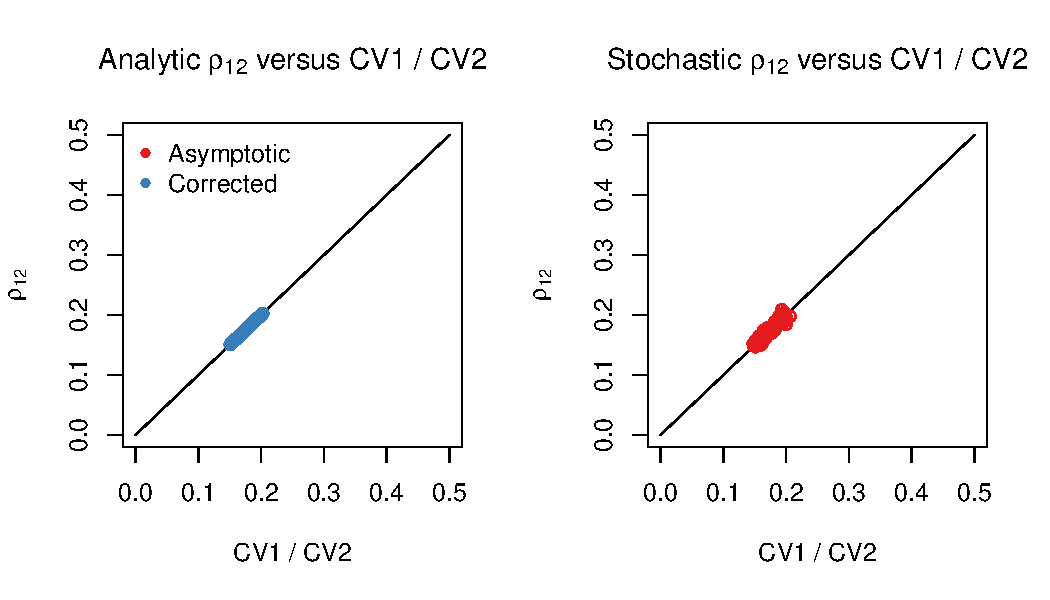
\includegraphics[width=\maxwidth]{../figures/twocolumn-cv_rel-1} 

}

\caption[ ]{ }\label{fig:cv_rel}
\end{figure}
\end{Schunk}



  
%   Combine the plot from Question 2C with your new stationary state simulations as well as the predicted
% relationship derived from Question 3E for your chosen values τ1, τ2. Comment on where
% your numerical simulations lie in relation to the previous systems with constant translation rate per
% mRNA: did the correlations go up or down? Did the ratio of CVs go up or down? Does this make
% intuitive sense?
  
  
\section{Acknowledgements}
  As always, many thanks to Julian Melgar for no particular reason. Also thanks to the people at Lund University who unwittingly lended me their computers for running the simulations.
  
\bibliography{references}
% \end{multicols*}

\newpage
\onecolumn
  \appendix
\section{Code}
   \lstinputlisting{../code/gillespie.sh}
   \lstinputlisting{../code/gillespie.R}
\end{document}
